% Generated by pysimcount.figgroupline -- do not edit; regenerate instead.
% figure: grouping-cnot-xyz-vs-twogroup-measured -- X-Y-Z vs two-group (even-out): r and CNOT count at measured n
% source: ../np-grouping/aggregate.json (seeds [1, 2, 3, 4, 5, 6, 7, 8, 9, 10]); merged, cz, simcount template
% shown: suzuki4, mo-q14, morales-m8, bm-q10; n = [4, 6, 8, 10]
% plotted: mean over seeds; bars min..max over seeds; all r measured
% r ratio at n=10 (mean X-Y-Z / mean two-group): (1.0030769230769232, 1.1147540983606559)
% CNOT ratio at n=10: (2.6366593406593406, 2.921424533634822)
% derived: ../np-grouping/aggregate.json; points equal main-cnot-all-formulas.json sha256=500e44d2dcd8af1b87c0e674b1bbfda8db5fe55c084698bcdf0ad96a67f293ce; grouping-cnot-twogroup-even-out.json sha256=ebe7fd4608a8dcd011da6adcdd4c0c0f5471b9f9f194be5cdaeeec8f862d7b64 (checked) by pysimcount.figgroupline
% figure made at git_commit=e5d9ee696f892e28aced765585653760f8a427c4 git_dirty=False
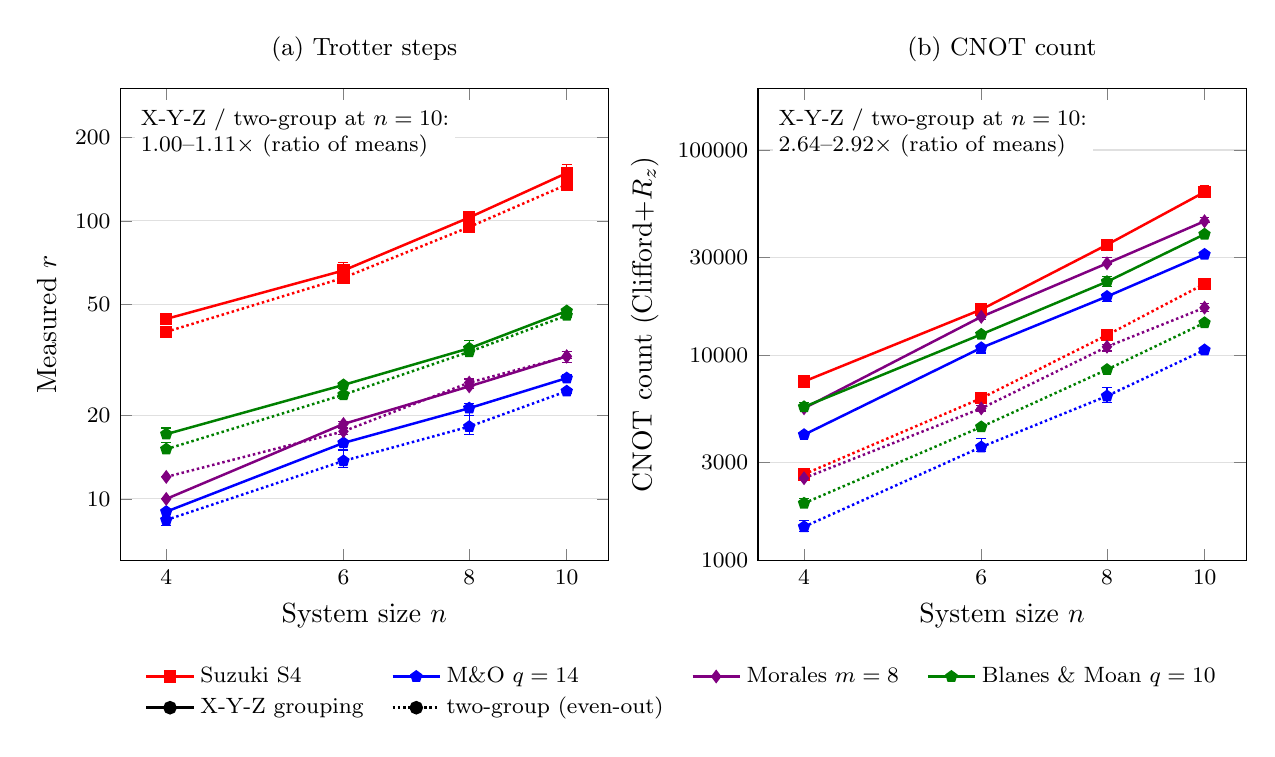
\begin{tikzpicture}
  \begin{loglogaxis}[
    scale only axis,
    at={(0cm,0cm)}, anchor=south west,
    width=6.2cm, height=6.0cm,
    title={(a) Trotter steps}, title style={font=\small},
    xlabel={System size $n$},
    ylabel={Measured $r$},
    xtick={4,6,8,10}, xticklabels={4,6,8,10}, xminorticks=false,
    ytick={10,20,50,100,200}, yticklabels={10,20,50,100,200}, yminorticks=false,
    xmin=3.6, xmax=11, ymin=6, ymax=300,
    ymajorgrids=true, grid style={black!12}, tick label style={font=\footnotesize},
  ]
    % suzuki4 xyz: mean over seeds, bars min..max over seeds
    \addplot[red, solid, line width=0.9pt, mark=square*, mark size=1.8pt, mark options={solid, fill=red}, forget plot, error bars/.cd, y dir=both, y explicit, error bar style={solid, line width=0.4pt}] coordinates {
      (4,44.4) += (0,0.6) -= (0,0.4)
      (6,66.3) += (0,4.7) -= (0,3.3)
      (8,102.8) += (0,4.2) -= (0,3.8)
      (10,148.6) += (0,11.4) -= (0,5.6)
    };
    % mo-q14 xyz: mean over seeds, bars min..max over seeds
    \addplot[blue, solid, line width=0.9pt, mark=pentagon*, mark size=1.8pt, mark options={solid, fill=blue}, forget plot, error bars/.cd, y dir=both, y explicit, error bar style={solid, line width=0.4pt}] coordinates {
      (4,9) += (0,0) -= (0,0)
      (6,15.9) += (0,0.1) -= (0,0.9)
      (8,21.2) += (0,0.8) -= (0,1.2)
      (10,27.2) += (0,0.8) -= (0,0.2)
    };
    % morales-m8 xyz: mean over seeds, bars min..max over seeds
    \addplot[violet, solid, line width=0.9pt, mark=diamond*, mark size=1.8pt, mark options={solid, fill=violet}, forget plot, error bars/.cd, y dir=both, y explicit, error bar style={solid, line width=0.4pt}] coordinates {
      (4,10) += (0,0) -= (0,0)
      (6,18.6) += (0,0.4) -= (0,0.6)
      (8,25.4) += (0,1.6) -= (0,0.4)
      (10,32.6) += (0,1.4) -= (0,0.6)
    };
    % bm-q10 xyz: mean over seeds, bars min..max over seeds
    \addplot[green!50!black, solid, line width=0.9pt, mark=pentagon*, mark size=1.8pt, mark options={solid, fill=green!50!black}, forget plot, error bars/.cd, y dir=both, y explicit, error bar style={solid, line width=0.4pt}] coordinates {
      (4,17.1) += (0,0.9) -= (0,0.1)
      (6,25.7) += (0,0.3) -= (0,0.7)
      (8,34.8) += (0,2.2) -= (0,1.8)
      (10,47.4) += (0,0.6) -= (0,1.4)
    };
    % suzuki4 twogroup-even-out: mean over seeds, bars min..max over seeds
    \addplot[red, densely dotted, line width=0.9pt, mark=square*, mark size=1.8pt, mark options={solid, fill=red}, forget plot, error bars/.cd, y dir=both, y explicit, error bar style={solid, line width=0.4pt}] coordinates {
      (4,39.9) += (0,1.1) -= (0,0.9)
      (6,62.4) += (0,0.6) -= (0,0.4)
      (8,95) += (0,1) -= (0,1)
      (10,135) += (0,3) -= (0,1)
    };
    % mo-q14 twogroup-even-out: mean over seeds, bars min..max over seeds
    \addplot[blue, densely dotted, line width=0.9pt, mark=pentagon*, mark size=1.8pt, mark options={solid, fill=blue}, forget plot, error bars/.cd, y dir=both, y explicit, error bar style={solid, line width=0.4pt}] coordinates {
      (4,8.4) += (0,0.6) -= (0,0.4)
      (6,13.7) += (0,1.3) -= (0,0.7)
      (8,18.2) += (0,1.8) -= (0,1.2)
      (10,24.4) += (0,0.6) -= (0,0.4)
    };
    % morales-m8 twogroup-even-out: mean over seeds, bars min..max over seeds
    \addplot[violet, densely dotted, line width=0.9pt, mark=diamond*, mark size=1.8pt, mark options={solid, fill=violet}, forget plot, error bars/.cd, y dir=both, y explicit, error bar style={solid, line width=0.4pt}] coordinates {
      (4,12) += (0,0) -= (0,0)
      (6,17.5) += (0,0.5) -= (0,0.5)
      (8,26.2) += (0,0.8) -= (0,1.2)
      (10,32.5) += (0,1.5) -= (0,1.5)
    };
    % bm-q10 twogroup-even-out: mean over seeds, bars min..max over seeds
    \addplot[green!50!black, densely dotted, line width=0.9pt, mark=pentagon*, mark size=1.8pt, mark options={solid, fill=green!50!black}, forget plot, error bars/.cd, y dir=both, y explicit, error bar style={solid, line width=0.4pt}] coordinates {
      (4,15.1) += (0,0.9) -= (0,0.1)
      (6,23.7) += (0,0.3) -= (0,0.7)
      (8,33.8) += (0,0.2) -= (0,0.8)
      (10,45.7) += (0,1.3) -= (0,0.7)
    };
    \node[anchor=north west, font=\footnotesize, fill=white, inner sep=2pt, align=left] at (rel axis cs:0.03,0.97) {X-Y-Z / two-group at $n=10$:\\1.00--1.11$\times$ (ratio of means)};
  \end{loglogaxis}
  \begin{loglogaxis}[
    scale only axis,
    at={(8.1cm,0cm)}, anchor=south west,
    width=6.2cm, height=6.0cm,
    title={(b) CNOT count}, title style={font=\small},
    xlabel={System size $n$},
    ylabel={CNOT count (Clifford+$R_z$)},
    xtick={4,6,8,10}, xticklabels={4,6,8,10}, xminorticks=false,
    ytick={1000,3000,10000,30000,100000}, yticklabels={1000,3000,10000,30000,100000}, yminorticks=false,
    xmin=3.6, xmax=11, ymin=1000, ymax=200000,
    ymajorgrids=true, grid style={black!12}, tick label style={font=\footnotesize},
    legend style={at={(-0.1532,-0.2)}, anchor=north, draw=none, font=\footnotesize,
      legend columns=4, /tikz/every even column/.append style={column sep=8pt}},
    legend cell align=left,
  ]
    % suzuki4 xyz: mean over seeds, bars min..max over seeds
    \addplot[red, solid, line width=0.9pt, mark=square*, mark size=1.8pt, mark options={solid, fill=red}, error bars/.cd, y dir=both, y explicit, error bar style={solid, line width=0.4pt}] coordinates {
      (4,7459.2) += (0,100.8) -= (0,67.2)
      (6,16707.6) += (0,1184.4) -= (0,831.6)
      (8,34540.8) += (0,1411.2) -= (0,1276.8)
      (10,62412) += (0,4788) -= (0,2352)
    };
    \addlegendentry{Suzuki S4}
    % mo-q14 xyz: mean over seeds, bars min..max over seeds
    \addplot[blue, solid, line width=0.9pt, mark=pentagon*, mark size=1.8pt, mark options={solid, fill=blue}, error bars/.cd, y dir=both, y explicit, error bar style={solid, line width=0.4pt}] coordinates {
      (4,4104) += (0,0) -= (0,0)
      (6,10875.6) += (0,68.4) -= (0,615.6)
      (8,19334.4) += (0,729.6) -= (0,1094.4)
      (10,31008) += (0,912) -= (0,228)
    };
    \addlegendentry{M\&O $q=14$}
    % morales-m8 xyz: mean over seeds, bars min..max over seeds
    \addplot[violet, solid, line width=0.9pt, mark=diamond*, mark size=1.8pt, mark options={solid, fill=violet}, error bars/.cd, y dir=both, y explicit, error bar style={solid, line width=0.4pt}] coordinates {
      (4,5520) += (0,0) -= (0,0)
      (6,15400.8) += (0,331.2) -= (0,496.8)
      (8,28041.6) += (0,1766.4) -= (0,441.6)
      (10,44988) += (0,1932) -= (0,828)
    };
    \addlegendentry{Morales $m=8$}
    % bm-q10 xyz: mean over seeds, bars min..max over seeds
    \addplot[green!50!black, solid, line width=0.9pt, mark=pentagon*, mark size=1.8pt, mark options={solid, fill=green!50!black}, error bars/.cd, y dir=both, y explicit, error bar style={solid, line width=0.4pt}] coordinates {
      (4,5608.8) += (0,295.2) -= (0,32.8)
      (6,12644.4) += (0,147.6) -= (0,344.4)
      (8,22828.8) += (0,1443.2) -= (0,1180.8)
      (10,38868) += (0,492) -= (0,1148)
    };
    \addlegendentry{Blanes \& Moan $q=10$}
    % suzuki4 twogroup-even-out: mean over seeds, bars min..max over seeds
    \addplot[red, densely dotted, line width=0.9pt, mark=square*, mark size=1.8pt, mark options={solid, fill=red}, forget plot, error bars/.cd, y dir=both, y explicit, error bar style={solid, line width=0.4pt}] coordinates {
      (4,2633.4) += (0,72.6) -= (0,59.4)
      (6,6177.6) += (0,59.4) -= (0,39.6)
      (8,12540) += (0,132) -= (0,132)
      (10,22275) += (0,495) -= (0,165)
    };
    % mo-q14 twogroup-even-out: mean over seeds, bars min..max over seeds
    \addplot[blue, densely dotted, line width=0.9pt, mark=pentagon*, mark size=1.8pt, mark options={solid, fill=blue}, forget plot, error bars/.cd, y dir=both, y explicit, error bar style={solid, line width=0.4pt}] coordinates {
      (4,1461.6) += (0,104.4) -= (0,69.6)
      (6,3575.7) += (0,339.3) -= (0,182.7)
      (8,6333.6) += (0,626.4) -= (0,417.6)
      (10,10614) += (0,261) -= (0,174)
    };
    % morales-m8 twogroup-even-out: mean over seeds, bars min..max over seeds
    \addplot[violet, densely dotted, line width=0.9pt, mark=diamond*, mark size=1.8pt, mark options={solid, fill=violet}, forget plot, error bars/.cd, y dir=both, y explicit, error bar style={solid, line width=0.4pt}] coordinates {
      (4,2520) += (0,0) -= (0,0)
      (6,5512.5) += (0,157.5) -= (0,157.5)
      (8,11004) += (0,336) -= (0,504)
      (10,17062.5) += (0,787.5) -= (0,787.5)
    };
    % bm-q10 twogroup-even-out: mean over seeds, bars min..max over seeds
    \addplot[green!50!black, densely dotted, line width=0.9pt, mark=pentagon*, mark size=1.8pt, mark options={solid, fill=green!50!black}, forget plot, error bars/.cd, y dir=both, y explicit, error bar style={solid, line width=0.4pt}] coordinates {
      (4,1902.6) += (0,113.4) -= (0,12.6)
      (6,4479.3) += (0,56.7) -= (0,132.3)
      (8,8517.6) += (0,50.4) -= (0,201.6)
      (10,14395.5) += (0,409.5) -= (0,220.5)
    };
    \addlegendimage{black, solid, line width=0.9pt, mark=*, mark options={solid, fill=black}}
    \addlegendentry{X-Y-Z grouping}
    \addlegendimage{black, densely dotted, line width=0.9pt, mark=*, mark options={solid, fill=black}}
    \addlegendentry{two-group (even-out)}
    \node[anchor=north west, font=\footnotesize, fill=white, inner sep=2pt, align=left] at (rel axis cs:0.03,0.97) {X-Y-Z / two-group at $n=10$:\\2.64--2.92$\times$ (ratio of means)};
  \end{loglogaxis}
\end{tikzpicture}
